Pour être sûrs que nos résultats sont fiables - et que ce n'est pas, par exemple, le modèle linguistique qui ne fonctionne pas - nous devons effectuer des tests de contrôle. Il s'agit essentiellement de comparer les textes Incel avec des textes qui n'ont rien à voir avec eux, pour comprendre comment cela affecte leur visualisation.\\

Dans ce cas, on a utilisé un jeu de données contenant des résumés d'articles du journal italien “ilpost”\footcite{ilpost2022}. Il a été créé par le \emph{Applied Recognition Technology Laboratory} (Arte-Lab), un laboratoire de recherché rattaché à l'Université de l'Insubrie (Varese, Italie). En particulier, on a utilisé la partie "train" du dataset, qui correspond 35.201 titres. À l'aide du même modèle sentence-BERT utilisé précédemment, on a créé des embedding. Ensuite, les embeddings que nous venons de créer ont été fusionnés avec ceux du jeu de données incel de départ et nous avons appliqué les techniques de réduction dimensionnelle mentionnées précédemment, PCA et UMAP. Les représentations graphiques des résultats sont présentées ci-dessous\footnote{Pour la représentation des points obtenus avec UMAP, une librairie graphique différente a été utilisée pour rendre la visualisation plus claire.}. Les points verts sont les phrases de contrôle et les points rouges sont les phrases incel.

\begin{figure}[h!]
	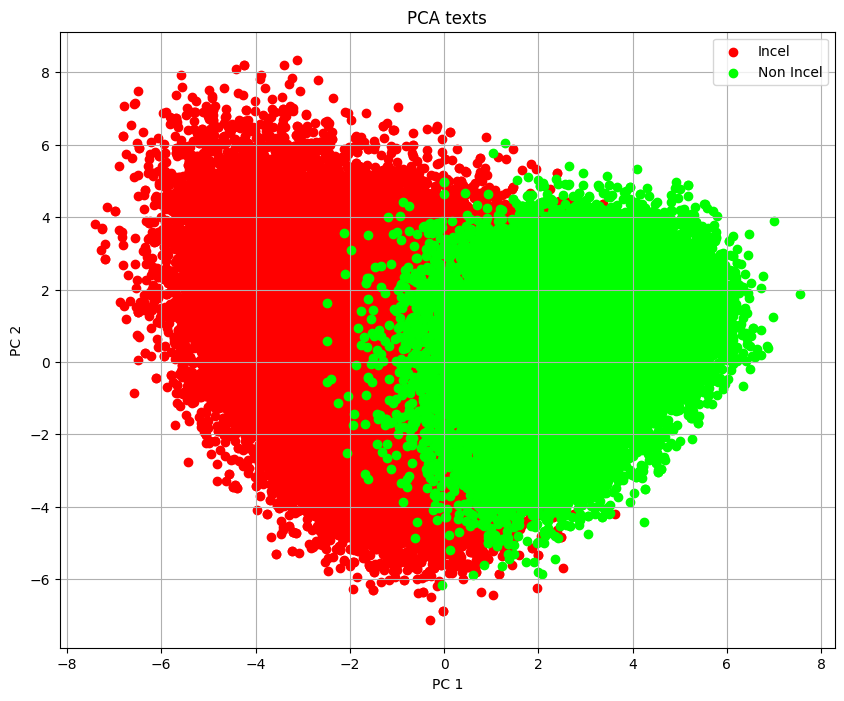
\includegraphics[scale=0.4]{PCA_test.png}
	\centering
	\caption{Plot des données réduites par PCA}
\end{figure}

\begin{figure}[h!]
	\includegraphics[scale=0.45]{umap_test.png}
	\centering
	\caption{Plot des données réduites par UMAP}
\end{figure}

\clearpage

Comme on peut le voir, les deux groupes peuvent être identifiés  assez facilement à partir des deux graphiques. 
Cela montre globalement que le modèle de langue utilisé fonctionne et que, par conséquent, le chevauchement presque complet des points dans les figures 1 et 2 peut être considéré comme une preuve de l'homogénéité du sens des phrases dans le dataset de départ.